\documentclass{beamer}
\mode<presentation>
\usepackage{amsmath}
\usepackage{amssymb}
%\usepackage{advdate}
\usepackage{adjustbox}
\usepackage{subcaption}
\usepackage{enumitem}
\usepackage{multicol}
\usepackage{mathtools}
\usepackage{listings}
\usepackage{url}
\def\UrlBreaks{\do\/\do-}
\usetheme{Boadilla}
\usecolortheme{lily}
\setbeamertemplate{footline}
{
  \leavevmode%
  \hbox{%
  \begin{beamercolorbox}[wd=\paperwidth,ht=2.25ex,dp=1ex,right]{author in head/foot}%
    \insertframenumber{} / \inserttotalframenumber\hspace*{2ex} 
  \end{beamercolorbox}}%
  \vskip0pt%
}
\setbeamertemplate{navigation symbols}{}

\providecommand{\nCr}[2]{\,^{#1}C_{#2}} % nCr
\providecommand{\nPr}[2]{\,^{#1}P_{#2}} % nPr
\providecommand{\mbf}{\mathbf}
\providecommand{\pr}[1]{\ensuremath{\Pr\left(#1\right)}}
\providecommand{\qfunc}[1]{\ensuremath{Q\left(#1\right)}}
\providecommand{\sbrak}[1]{\ensuremath{{}\left[#1\right]}}
\providecommand{\lsbrak}[1]{\ensuremath{{}\left[#1\right.}}
\providecommand{\rsbrak}[1]{\ensuremath{{}\left.#1\right]}}
\providecommand{\brak}[1]{\ensuremath{\left(#1\right)}}
\providecommand{\lbrak}[1]{\ensuremath{\left(#1\right.}}
\providecommand{\rbrak}[1]{\ensuremath{\left.#1\right)}}
\providecommand{\cbrak}[1]{\ensuremath{\left\{#1\right\}}}
\providecommand{\lcbrak}[1]{\ensuremath{\left\{#1\right.}}
\providecommand{\rcbrak}[1]{\ensuremath{\left.#1\right\}}}
\theoremstyle{remark}
\newtheorem{rem}{Remark}
\newcommand{\sgn}{\mathop{\mathrm{sgn}}}
\providecommand{\abs}[1]{\left\vert#1\right\vert}
\providecommand{\res}[1]{\Res\displaylimits_{#1}} 
\providecommand{\norm}[1]{\lVert#1\rVert}
\providecommand{\mtx}[1]{\mathbf{#1}}
\providecommand{\mean}[1]{E\left[ #1 \right]}
\providecommand{\fourier}{\overset{\mathcal{F}}{ \rightleftharpoons}}
%\providecommand{\hilbert}{\overset{\mathcal{H}}{ \rightleftharpoons}}
\providecommand{\system}{\overset{\mathcal{H}}{ \longleftrightarrow}}
	%\newcommand{\solution}[2]{\textbf{Solution:}{#1}}
%\newcommand{\solution}{\noindent \textbf{Solution: }}
\providecommand{\dec}[2]{\ensuremath{\overset{#1}{\underset{#2}{\gtrless}}}}
\newcommand{\myvec}[1]{\ensuremath{\begin{pmatrix}#1\end{pmatrix}}}
\newcommand{\mydet}[1]{\ensuremath{\begin{vmatrix}#1\end{vmatrix}}}
\let\vec\mathbf

\lstset{
%language=C,
frame=single, 
breaklines=true,
columns=fullflexible
}

\numberwithin{equation}{section}

\title{4.11.34}
\author{Rushil Shanmukha Srinivas \\EE25BTECH11057 \\ Electrical Enggineering ,\\IIT Hyderabad.}

\date{\today} 
\begin{document} 

\begin{frame}
\titlepage
\end{frame}

\section*{Outline}
\begin{frame}
\tableofcontents
\end{frame}
\section{Problem}
\begin{frame}
\frametitle{Problem Statement}
\textbf{Question} : Find the area of the region bounded by the lines 3x-2y+1=0,2x+3y-21=0 and x-5y+9=0 .

\end{frame}
\section{Solution}
\subsection{Obtaining Vertices and Finding Area}
\begin{frame}
\frametitle{Obtaining Vertices and Finding Area}
%\framesubtitle{Literature}
\textbf{Solution:}
Given three lines are
\begin{align}
\myvec{3 & -2}\myvec{x\\y} = -1 \Longrightarrow \vec{n}^\top\vec{x} = -1
\end{align}
\begin{align}
\myvec{2 & 3}\myvec{x\\y} = 21 \Longrightarrow \vec{m}^\top\vec{x} = 21
\end{align}
\begin{align}
\myvec{1 & -5}\myvec{x\\y} = -9 \Longrightarrow \vec{p}^\top\vec{x} = -9
\end{align}
The three lines form a triangle.
The vertices of triangle are obtained by 
\textbf{Intersection of :}
\begin{align}
\vec{n}^\top\vec{x} = -1 \ and \ \vec{m}^\top\vec{x} = 21 
\end{align}
The augmented system in matrix form is

\begin{align}
\myvec{
3 & -2 &\vrule& -1\\
2 & 3 &\vrule& 21} \xrightarrow{R_2 \longrightarrow 3R_2-2R_1}
\myvec{
3 & -2 &\vrule& -1\\
0 & 13 &\vrule& 65}
\end{align}
\end{frame}
\begin{frame}
$ From \ the \ second \ row \ we \ get\ y=5 \ so \ x=3 \Longrightarrow
\vec{A} = \myvec{3\\5}$

\begin{align}
\vec{m}^\top\vec{x} = 21 \ and \ \vec{p}^\top\vec{x} = -9
\end{align}
The augmented matrix is

\begin{align}
\myvec{
2 & 3 &\vrule& 21\\
1 & -5 &\vrule& -9} \xrightarrow{R_2 \longrightarrow 2R_2-R_1}
\myvec{
2 & 3 &\vrule& 21\\
0 & -13 &\vrule& -39}
\end{align}
$ From \ the \ second \ row \ we \ get\ y=3 \ so \ x=6 \Longrightarrow
\vec{B} = \myvec{6\\3} $

\begin{align}
\vec{p}^\top\vec{x} = -9 \ and \ \vec{n}^\top\vec{x} = -1 
\end{align}
The augmented matrix is

\begin{align}
\myvec{
1 & -5 &\vrule& -9\\
3 & -2 &\vrule& -1} \xrightarrow{R_2 \longrightarrow R_2-3R_1}
\myvec{
1 & -5 &\vrule& -9\\
0 & 13 &\vrule& 26}
\end{align}
$ From \ the \ second \ row \ we \ get \ y=2 \ so \ x=1 \Longrightarrow
\vec{C} = \myvec{1\\2} $
\end{frame}
\begin{frame}
\begin{align}
\vec{A}-\vec{B} = \myvec{-3\\2} , \vec{A}-\vec{C} = \myvec{2\\3}   
\end{align}
\begin{align}
\norm{(\vec{A}-\vec{B})\times(\vec{A}-\vec{C})} =|\mydet{-3 & 2 \\
2 & 3}| = |-9-4| =|-13| = 13
\end{align}
\begin{align}
Area \ of \ the \ triangle = \frac{1}{2}{\norm{(\vec{A}-\vec{B})\times(\vec{A}-\vec{C}}}
                            =\frac{13}{2}
\end{align}

\end{frame}
\subsection{Plots}
\begin{frame}
\frametitle{Plots}
\begin{figure}
\centering
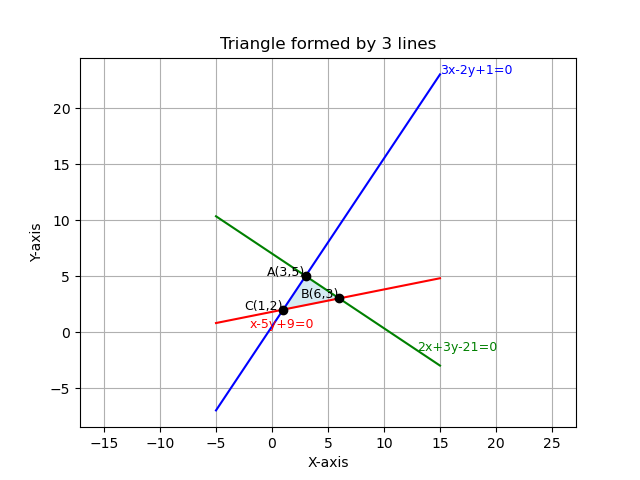
\includegraphics[width=0.9\columnwidth]{figs/fig8.png}
\caption{fig : Representation of Triangle}
\label{Fig8}
\end{figure}
\end{frame}
\section{C Code}
\begin{frame}[fragile]
\frametitle{C Code }
\begin{lstlisting}[language=C]  
#include <stdio.h>
#include <stdlib.h>
#include <math.h>

void solveIntersection(double a1,double b1,double c1,
                       double a2,double b2,double c2,
                       double *x,double *y) {
    double det = a1*b2 - a2*b1;
    *x = (b1*(-c2) - b2*(-c1)) / det;
    *y = (a2*(-c1) - a1*(-c2)) / det;}
double triangleArea() {
    double x1,y1,x2,y2,x3,y3;

    // Line1 & Line2
    solveIntersection(3,-2,1, 2,3,-21,&x1,&y1);
    // Line2 & Line3
    solveIntersection(2,3,-21, 1,-5,9,&x2,&y2);
\end{lstlisting}
\end{frame}
 \begin{frame}[fragile]
\begin{lstlisting}
    // Line1 & Line3
    solveIntersection(3,-2,1, 1,-5,9,&x3,&y3);

    double area = 0.5 * fabs(x1*(y2-y3) + x2*(y3-y1) + x3*(y1-y2));
    return area;
}

\end{lstlisting}
\end{frame}

\section{Python Code}
\begin{frame}[fragile]
\frametitle{Python : call\_c.py}
\begin{lstlisting}
import ctypes
import os

# Path to the compiled shared object
lib_path = os.path.abspath("./libtriangle.so")

# Load the shared library
lib = ctypes.CDLL(lib_path)

# Specify return type of the triangleArea function
lib.triangleArea.restype = ctypes.c_double

# Call the C function
area = lib.triangleArea()
# Print the solution
print("The area of the triangle formed by the given lines is:", area)

\end{lstlisting}
\end{frame}

\begin{frame}[fragile]
\frametitle{Python Code for Plotting}
\begin{lstlisting}[language=Python]
import numpy as np
import matplotlib.pyplot as plt

# Solve intersection of two lines ax + by + c = 0
def intersection(a1,b1,c1, a2,b2,c2):
    A = np.array([[a1,b1],[a2,b2]])
    B = np.array([-c1,-c2])
    x, y = np.linalg.solve(A,B)
    return x, y

# Line equations
# 1) 3x - 2y + 1 = 0
# 2) 2x + 3y - 21 = 0
# 3) x - 5y + 9 = 0

# Find vertices
A = intersection(3,-2,1, 2,3,-21)
\end{lstlisting}
\end{frame}
\begin{frame}[fragile]
\begin{lstlisting}
B = intersection(2,3,-21, 1,-5,9)
C = intersection(3,-2,1, 1,-5,9)

x1,y1 = A
x2,y2 = B
x3,y3 = C
# Triangle vertices for plotting
triangle_x = [x1, x2, x3, x1]
triangle_y = [y1, y2, y3, y1]

# Plotting range
x_vals = np.linspace(-5, 15, 400)

# Line 1: 3x - 2y + 1 = 0 -> y = (3x+1)/2
y1_line = (3*x_vals + 1)/2
plt.plot(x_vals, y1_line, color="blue")
plt.text(15, (3*15+1)/2, "3x-2y+1=0", fontsize=9, color="blue")  # moved right
\end{lstlisting}
\end{frame}
\begin{frame}[fragile]
\begin{lstlisting}

# Line 2: 2x + 3y - 21 = 0 -> y = (21-2x)/3
y2_line = (21 - 2*x_vals)/3
plt.plot(x_vals, y2_line, color="green")
plt.text(13, (21-2*13)/3, "2x+3y-21=0", fontsize=9, color="green")

# Line 3: x - 5y + 9 = 0 -> y = (x+9)/5
y3_line = (x_vals + 9)/5
plt.plot(x_vals, y3_line, color="red")
plt.text(-2, ((-2+9)/5) - 1.0, "x-5y+9=0", fontsize=9, color="red")  # moved down

# Plot triangle
plt.fill(triangle_x, triangle_y, color="lightblue", alpha=0.5)

# Mark vertices
plt.scatter([x1,x2,x3],[y1,y2,y3], color="black", zorder=5)
\end{lstlisting}
\end{frame}
\begin{frame}[fragile]
\begin{lstlisting}
plt.text(x1,y1,f"A({int(round(x1))},{int(round(y1))})", fontsize=9, ha="right")
plt.text(x2,y2,f"B({int(round(x2))},{int(round(y2))})", fontsize=9, ha="right")
plt.text(x3,y3,f"C({int(round(x3))},{int(round(y3))})", fontsize=9, ha="right")

plt.xlabel("X-axis")
plt.ylabel("Y-axis")
plt.title("Triangle formed by 3 lines")
plt.grid(True)
plt.axis("equal")
plt.savefig("../figs/fig8.png")
plt.show()

\end{lstlisting}
\end{frame}

\end{document}
  
